\subsubsection{Door detection}
In order to isolate every room each door is detected and drawn onto a pixelshademap (a grayscale image object).

To locate a door a brushfire map (an object containing brushfire values for all coordinates) is created. 
In figure \ref{door_detections_steps} the stages of detection is shown for an area that contains three doors.
To better illustrate this detection each brushfire value is multiplied by ten.

In figure \ref{intersections} the door detection is going through the brushfire map and looking for where two waves meet.
When the waves meet a T section is formed and this is detectable in the map. 
In the direction of the T there is potentially a door as shown in figure \ref{possible_doors}

In figure \ref{correct_doors} the list of doors is narrowed down by checking if they have an obstacle on both sides in the distance correlating to the brushfire value.

To separate the rooms every door step is painted from the door until it meets an obstacle as shown in figure \ref{door_steps}.

\begin{figure}[ht]
\centering
  \begin{subfigure}[t]{0.3\textwidth}
    
\includegraphics[width = \textwidth]{graphics/doors_in_map}
    \caption{The map zoomed in to an area with doors.}
    \label{doors_in_map}
  \end{subfigure}
  \begin{subfigure}[t]{0.3\textwidth}
    
\includegraphics[width = \textwidth]{graphics/brushfire_door}
    \caption{Brushfire in an area that contains doors.}
    \label{brush_door}
  \end{subfigure}
  \begin{subfigure}[t]{0.3\textwidth}
    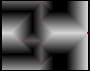
\includegraphics[width = \textwidth]{graphics/door_intersection}
    \caption{The T intersections viewed in the brushfire.}
    \label{intersections}
  \end{subfigure}
  \begin{subfigure}[t]{0.3\textwidth}
    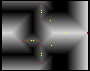
\includegraphics[width = \textwidth]{graphics/possible_doors}
    \caption{Possible doors in relation to the T sections.}
    \label{possible_doors}
  \end{subfigure}
  \begin{subfigure}[t]{0.3\textwidth}
    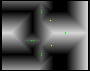
\includegraphics[width = \textwidth]{graphics/correct_doors}
    \caption{The correct doors.}
    \label{correct_doors}
  \end{subfigure}
  \begin{subfigure}[t]{0.3\textwidth}
    
\includegraphics[width = \textwidth]{graphics/door_steps}
    \caption{The door steps.}
    \label{door_steps}
  \end{subfigure}
\caption{Door detection step by step.}
\label{door_detections_steps}
\end{figure}